 
\section{Metodología}

\subsection{Obtención de datos}

El proceso de obtención de datos se realizó tomando imágenes satelitales que provee el satélite
Landsat 7. En este proceso se descargaron 1362 imágenes satelitales desde el año 1999 hasta el año 2015, que cubren el 
departamento de Nariño. Para cubrir todo el departamento fue necesario descargar las imagenes satelitales con 
los siguientes paths y rows: (009,059), (009,060), (010,058), (010,059), (011,059) 

En la obtención de datos también se utilizó el mapa de biomass construido por \cite{baccini2012estimated} 
construido para el año 2000 a 2003.


\subsection{Preprocesamiento}

En esta etapa de preprocesamiento se reproyecto las imágenes obtenidas, debido a que las cinco imágenes
que cubren el departamento de Nariño, estan en distintos sistemas de coordenadas (EPSG:32618 y EPSG:32617) y se 
lo reproyecto al sitema EPSG:3857. Así como también se recorto las imágenes con el fin de unicamente tener 
el área que cubre el departamento de Nariño, como lo muestra la figura~\ref{fig:Recortar imágenes}

\begin{figure}
  \centering
  \subfigure[Imágenes Satélitales de Nariño]{\label{Imágenes Satélitales Nariño} 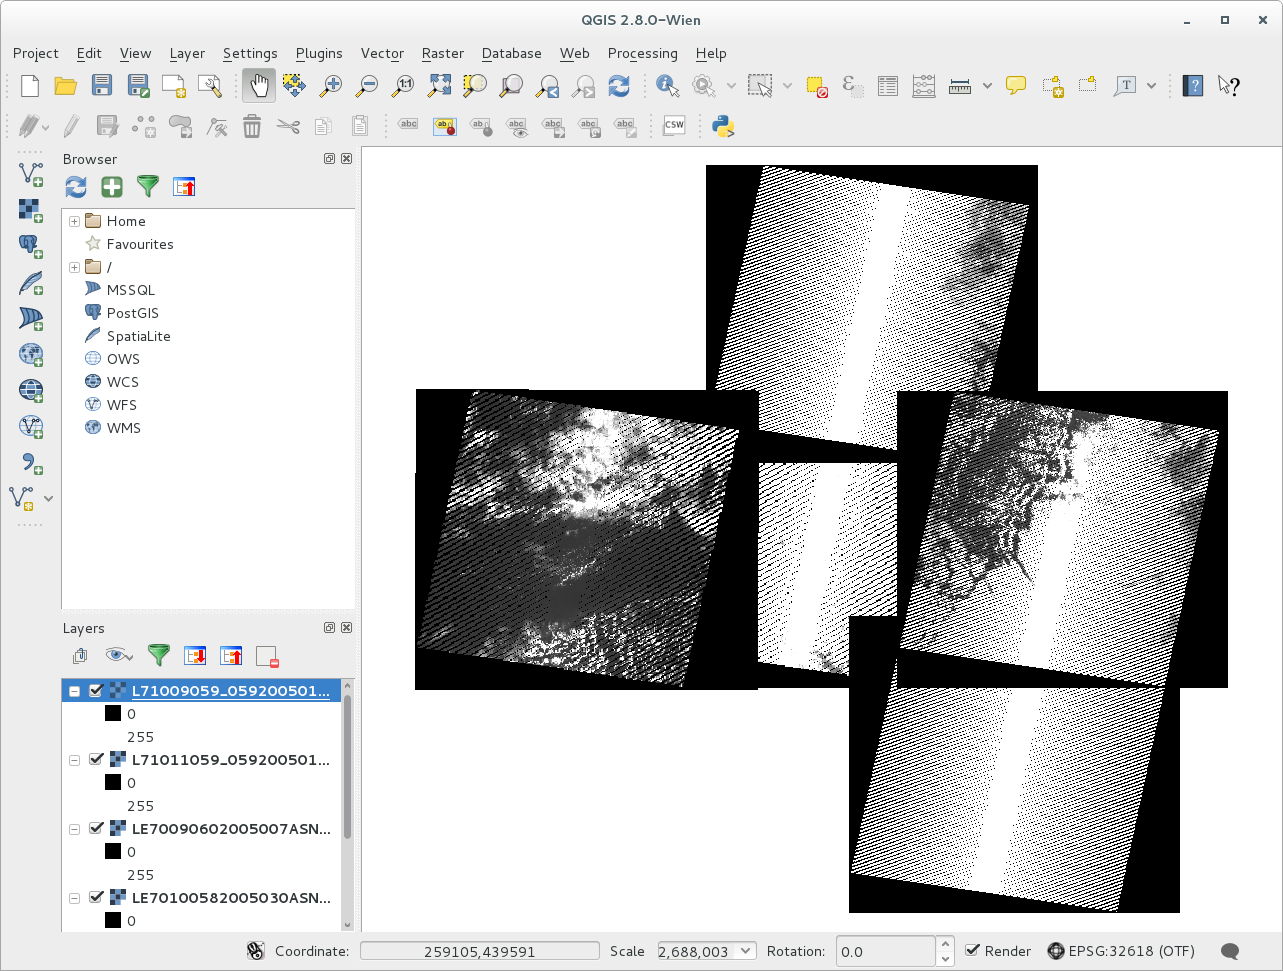
\includegraphics[width= 7cm]{cut1.png}}
  \vfill
  \subfigure[Imágenes recortadas de Nariño]{\label{Imágenes recortadas de Nariño}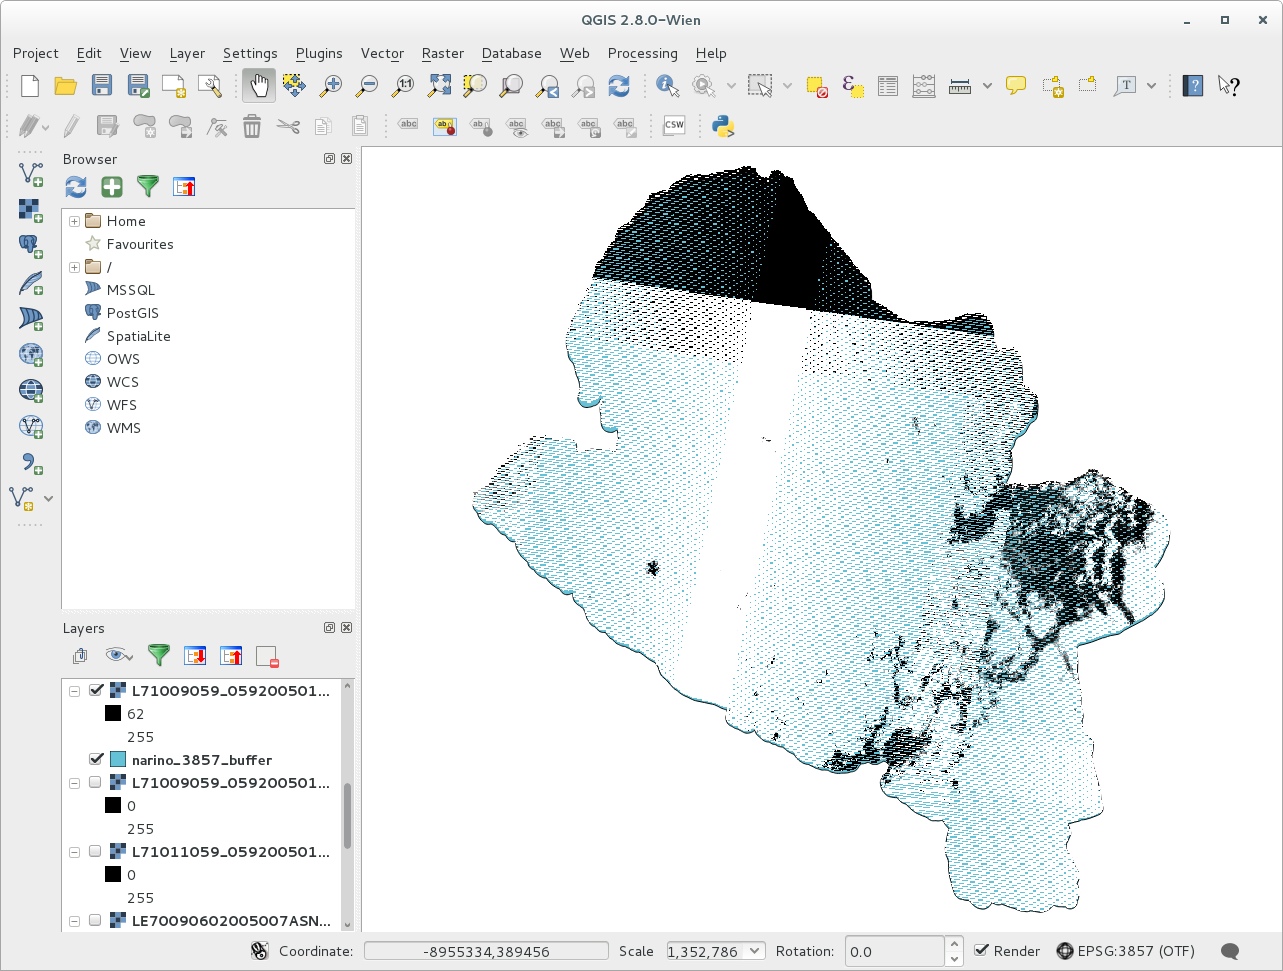
\includegraphics[width= 7cm]{cut2.png}}
  \caption{Prepocesamiento}
  \label{fig:Recortar imágenes}
\end{figure}

De igual manera este proceso se lo realizó para el mapa de biomasa, como se muestra en la figura~\ref{fig:mapaNarino}

\begin{figure}
  \centering
  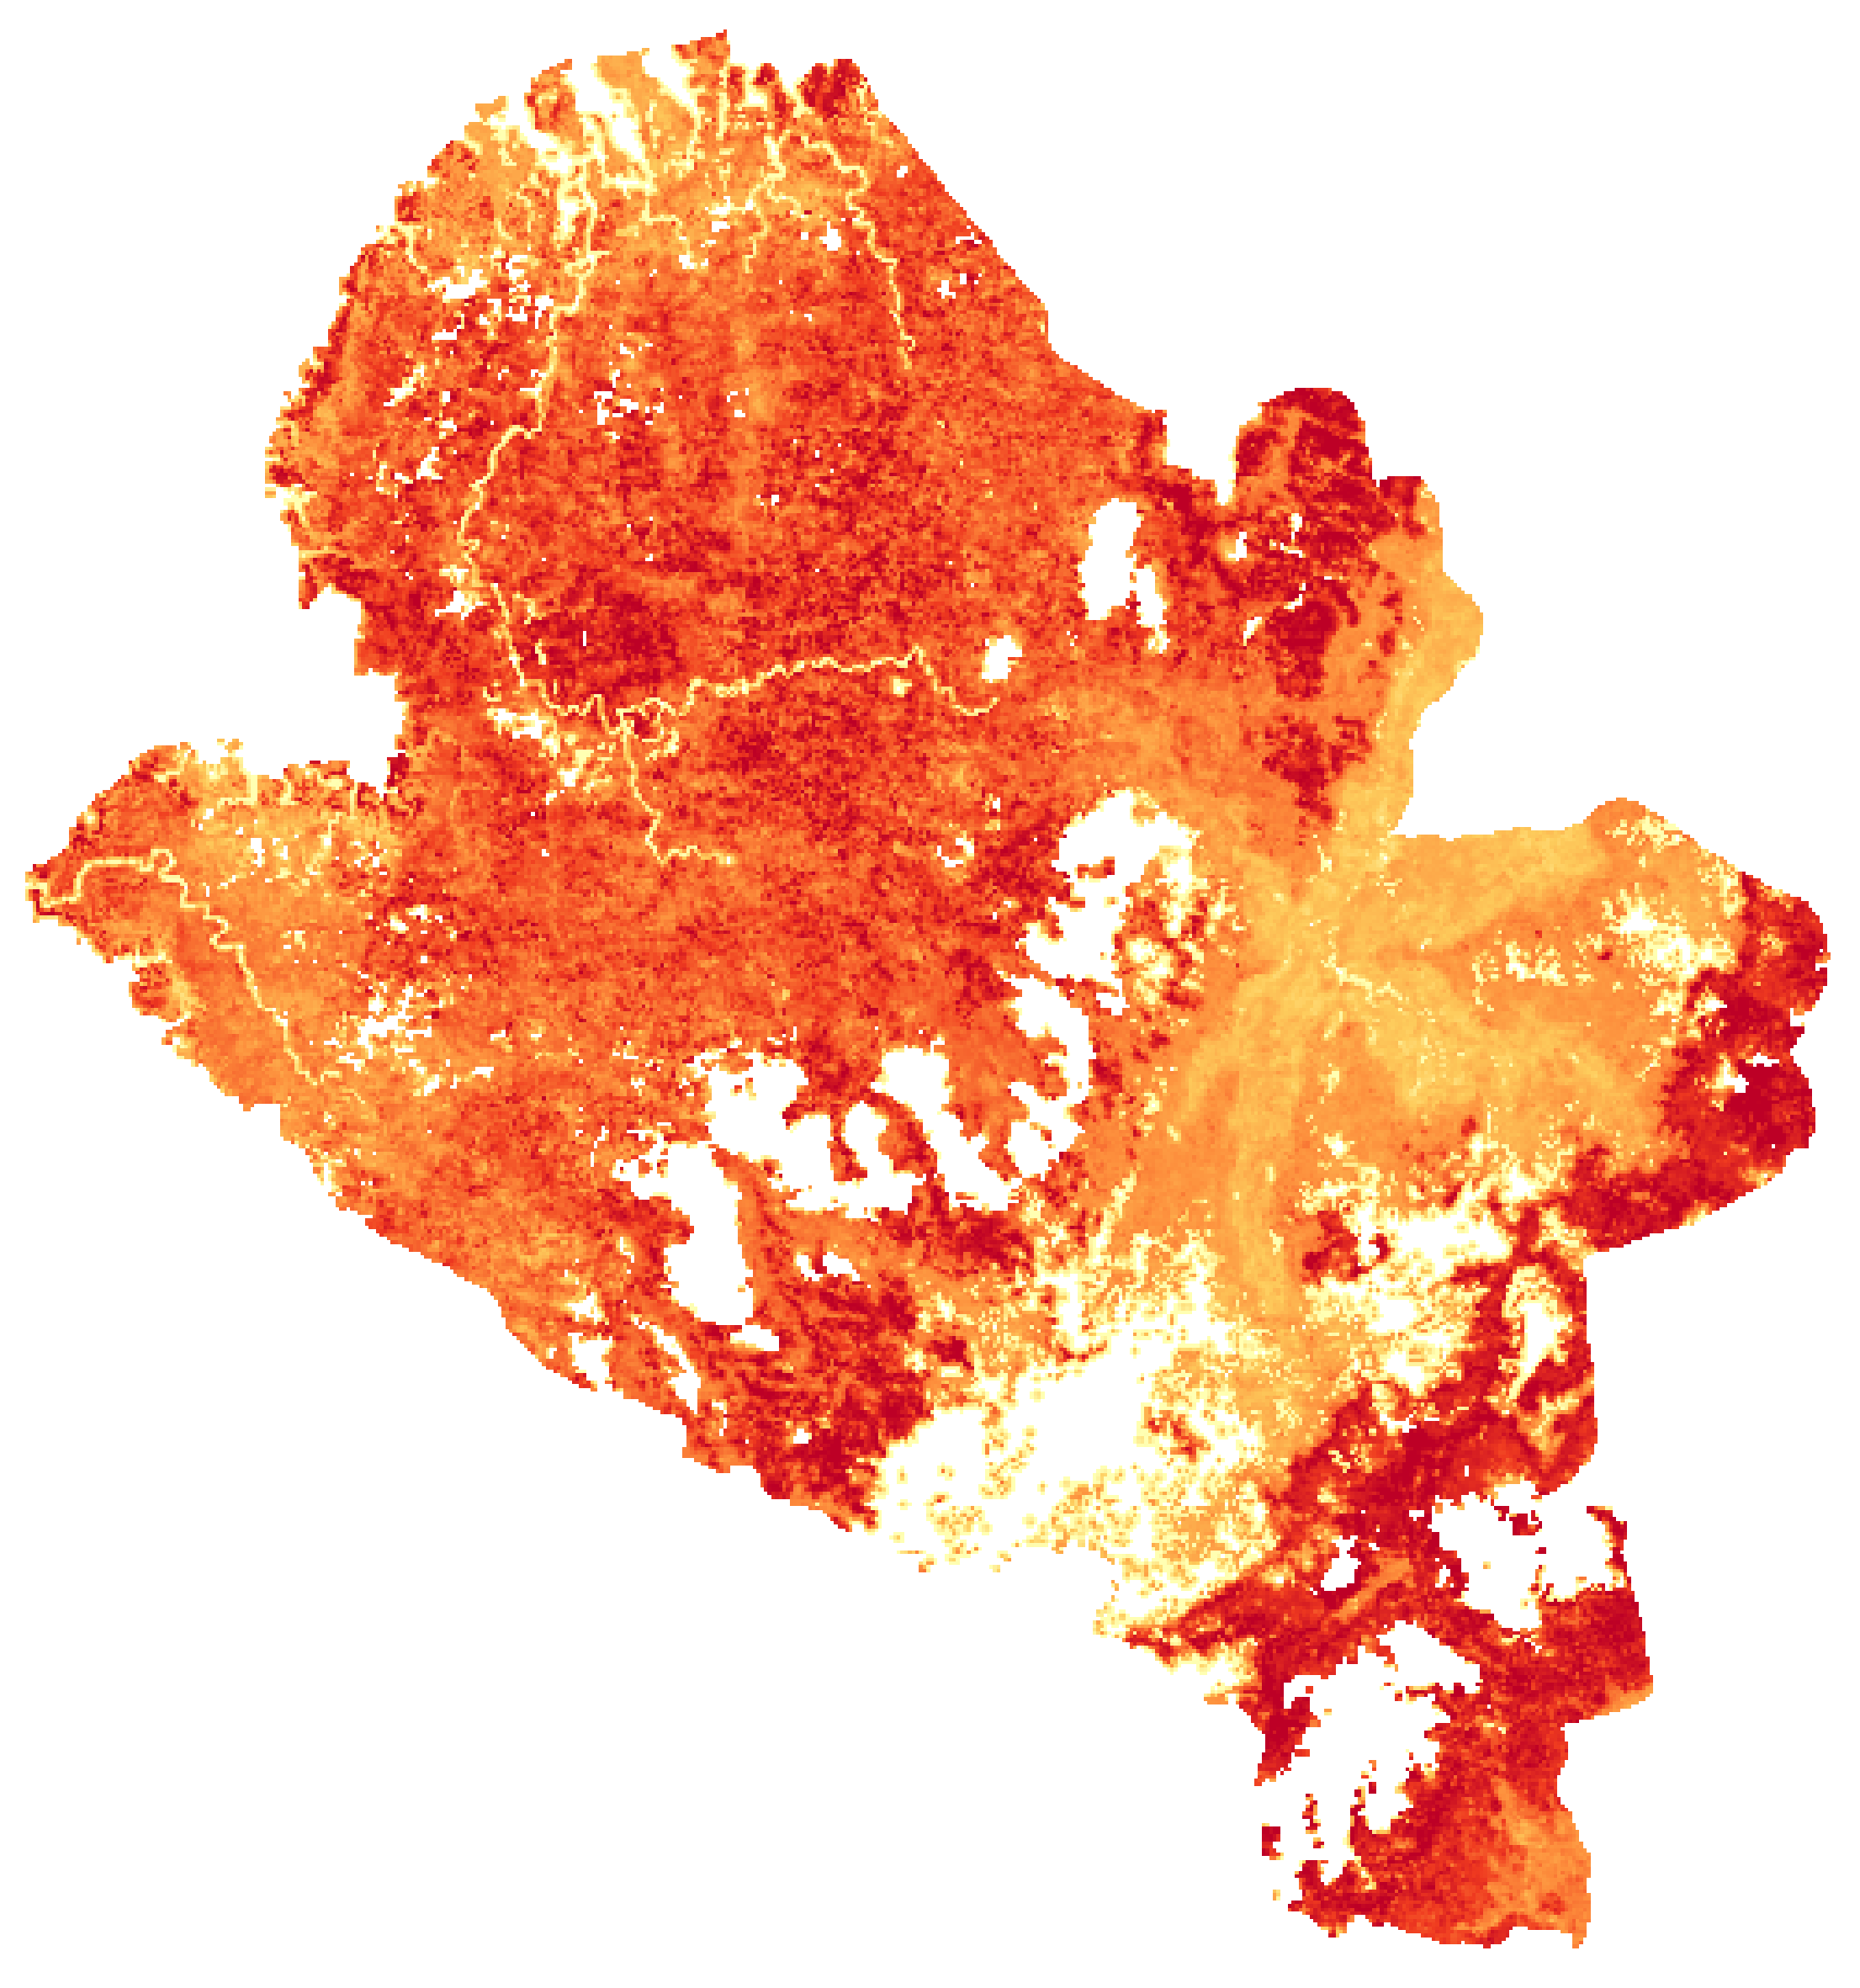
\includegraphics[width = 7cm]{mapaNarino.png}
  \caption{Mapa de biomasa en Nariño \cite{baccini2012estimated}}
  \label{fig:mapaNarino}
\end{figure}

\subsection{Procesamiento y limpieza de datos}

Para esta etapa, primero se diseño una base de datos para capturar los datos,
como lo muestra la figura~\ref{fig:landsatET}, la cual tiene 4 tablas. 

\begin{figure}
  \centering
  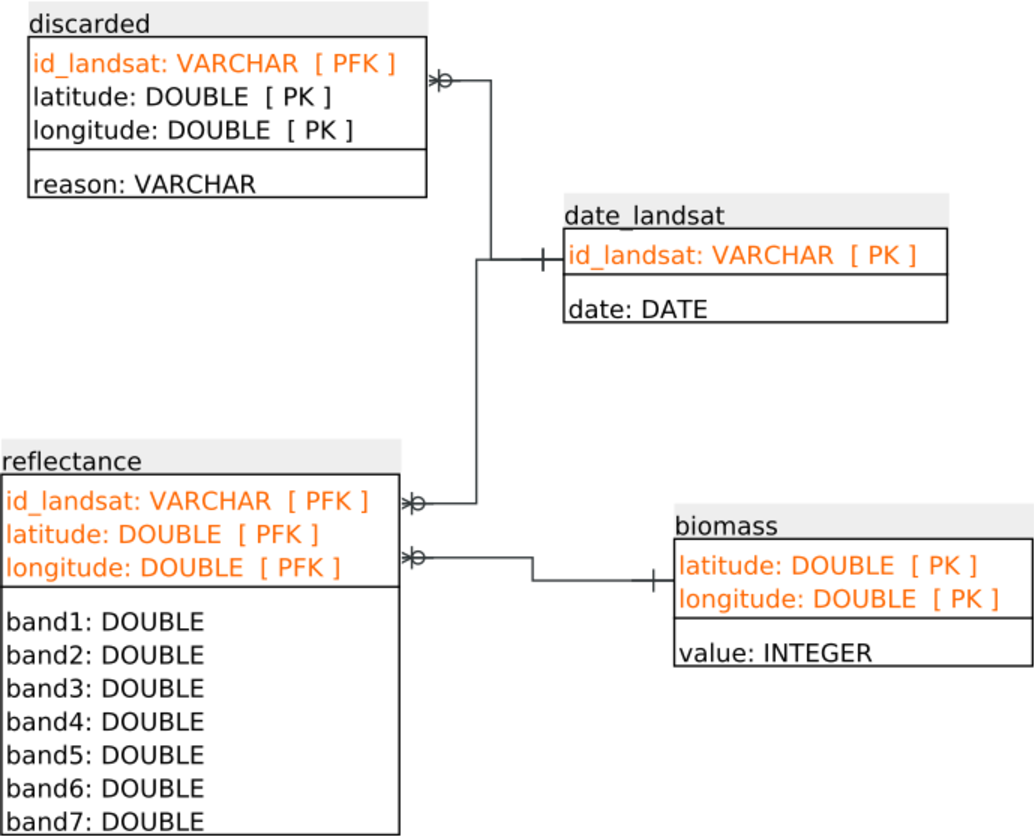
\includegraphics[width = 9cm]{landsatET.pdf}
  \caption{Modelo entidad-relacion Landsat}
  \label{fig:landsatET}
\end{figure}

Tabla date\_landsat: en la cual se almacenan las fechas de las imágenes satelitales.

Tabla reflectance: en la cual se almacenan los datos capturados y convertidos en reflentance,
de las bandas landsat (1 - 5,7) y la temperatura en grados kelvin de la banda 6.

Tabla discarded: en la cual se almacenan datos que fueron descartados, por varias razones,
son nubes calientes, nubes frias, datos ambiguos o no son vegetación.

Tabla biomass: en la cual se almacenan los datos de biomassa del mapa de \cite{baccini2012estimated}.

Para procesar las imágenes y llenar la base de datos se realizó un Script, el cual captura el Digital Number
de las imágenes satélitales y lo transforma en valor en reflectance. En este procesamiento de imagenes, se adiciono al Script unos filtros para para detección de nubes calientes,
nubes, frias, datos ambiguos como lo muestra el algoritmo propuesto por \cite{irish2000landsat}, además se aplico 
un filtro adicional, el NVDI(normalized difference vegetation index) para trabajar unicamente con datos de vegetación.

En la tabla XX se muestra una relación de los datos obtenidos.

\begin{table}
\caption{Datos obtenidos en en el proceso de procesamiento y limpieza  de datos}
\label{tab:metricas}
\centering
\scalebox{0.7}{
\begin{tabular}{c c c}
\toprule
 Nombre & Valor& Detalle  \\
\midrule
Imágenes landsat procesadas & 1321 & Imágenes de Nariño de 2000 a 2014 \\
Datos Totales & 51.076.512 & Registros Totales desde año 2000 a 2014 \\
Datos biomasa & 81.993 & Registros de biomasa para año 2000 a 2003 de  \cite{baccini2012estimated}\\
Nube caliente & 3.731.768 & Registros de 2000 a 2014 \\
Nube Fria & 27.827.009 & Registros de 2000 a 2014 \\
No vegetacion & 3.459.210 & Registros de 2000 a 2014 \\
Ambiguo & 11.987.340 & Registros de 2000 a 2014 \\
Datos Validos Reflectance & 4.071.185 & Registros de 2000 a 2014 \\

\bottomrule
\end{tabular}}
\end{table}



\subsection{Análisis de regresión}

El análisis de regresión se realizó tomando los valores de las bandas landsat obtenidas año 2000 y 2003 y el valor de biomasa obtenido en \cite{baccini2012estimated},
para poder obtener un mejor modelo se agrupó y se saco un promedio con valores de las bandas landsat en cada punto, se fue iterando con  valores que superaban al menos N número de
muestras, siendo N desde 1 hasta 45 muestras, el mejor modelo obtenido fué cuando el número de muestas en cada punto superaba al menos las 35 muestras, este conjunto
de datos obtenido tenía 1009 registros. El comportamiento en las demás iteraciones muestra que con menos muestras hay más registros y eso hace que no se encuentre un buen modelo,
pero cuando hay mas muestras los registros son menores y esto también hace que el resultado del modelo tampoco sea bueno.

En la tabla~\ref{tab:metricas} se muestra las métricas de los modelos analizadas con 35 muestras y 1009 datos, el cual es el mejor modelo, esta tabla 
se la realizó usando la biblioteca de código abierto rminer presentada por \cite{cortez2010data} para la herramienta R.

\begin{table}
\caption{Métricas de modelos analizados con 35 muestras y 1009 datos}
\label{tab:metricas}
\centering
\scalebox{0.7}{
\begin{tabular}{c c c c c c c}
\toprule
 & SAE& MAE & RAE & RMSE & COR & R2 \\
\midrule
ctree & 10406.58225 & 30.88007 & 65.04650 & 40.02893 & 0.69401 & 0.48165 \\
rpart & 10197.95826 & 30.26100 & 63.74249 & 39.37592 & 0.70520 & 0.49730 \\
kknn & 9147.51425 & 27.14396 & 57.17667 & 36.86581 & 0.74955 & 0.56182 \\
mlp & 9179.79310 & 27.23974 & 57.37843 & 34.70711 & 0.78122 & 0.61031 \\
mlpe & 8746.27740 & 25.95335 & 54.66874 & 34.57953 & 0.78309 & 0.61323 \\
ksvm & \textbf{8462.61487} & \textbf{25.11162} & \textbf{52.89570} & 34.67742 & \textbf{0.79830} & \textbf{0.63729} \\
randomForest & 8807.76477 & 26.13580 & 55.05306 & 34.70615 & 0.78239 & 0.61214 \\
mr & 10410.13919 & 30.89062 & 65.06873 & 38.61068 & 0.72000 & 0.51840 \\
mars & 8842.91866 & 26.24011 & 55.27279 & \textbf{33.96852} & 0.79161 & 0.62665 \\
cubist & 9012.54150 & 26.74345 & 56.33302 & 35.70576 & 0.77611 & 0.60235 \\
pcr & 10337.63121 & 30.67546 & 64.61552 & 38.59290 & 0.72023 & 0.51873 \\
plsr & 10337.63121 & 30.67546 & 64.61552 & 38.59290 & 0.72023 & 0.51873 \\
cppls & 10337.63121 & 30.67546 & 64.61552 & 38.59290 & 0.72023 & 0.51873 \\
\bottomrule
\end{tabular}}
\end{table}

En este proceso tambien se usó el paquete R Boruta \cite{kursa2010feature}, el cual es un nuevo algoritmo de selección de características 
para encontrar todas las variables relevantes. El algoritmo está diseñado como un recubrimiento alrededor 
del algoritmo de clasificación random forest. Esto para saber si todas las bandas de landsat utilizadas eran relevantes para encontrar biomasa, 
en la figura~\ref{fig:boruta} se puede observar la relevancia de las bandas landsat para encontrar biomasa en el mejor modelo.

\begin{figure}
  \centering
  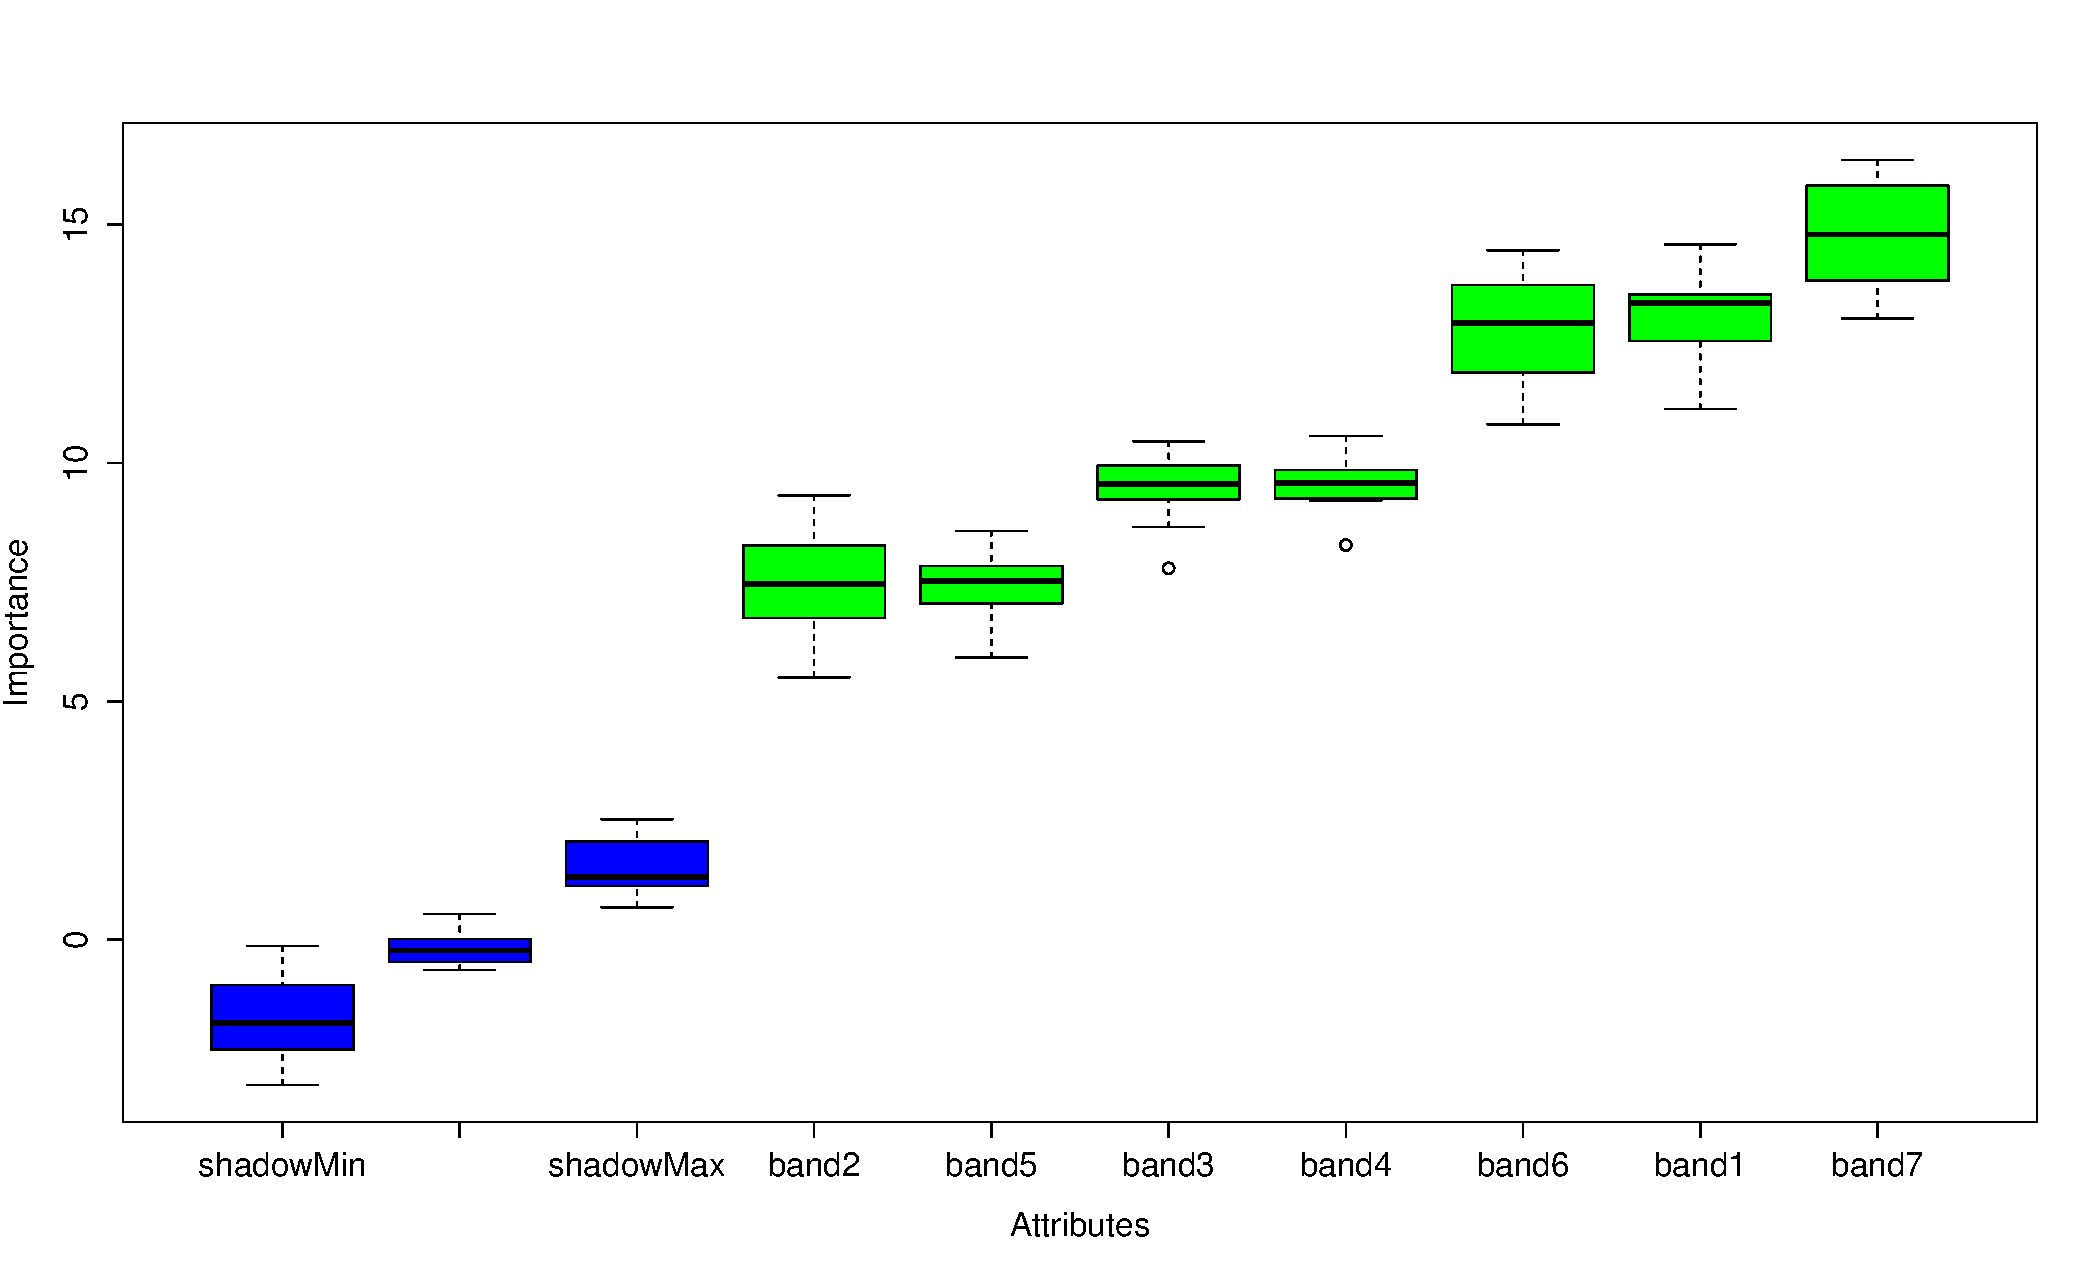
\includegraphics[width = 9cm]{boruta.pdf}
  \caption{Relevancia de bandas landsat en el análisis de regresión}
  \label{fig:boruta}
\end{figure}








